%% ============================================================
%%  Physics-Informed Neural Networks and Quantum Dot Systems
%%  Workshop talk — Beamer, aspectratio 169
%%  Author: Morten Hjorth-Jensen, UiO
%% ============================================================
\documentclass[aspectratio=169,10pt]{beamer}

% ── Theme ────────────────────────────────────────────────────────────────────
\usetheme{Madrid}
\usecolortheme{seahorse}
\setbeamertemplate{navigation symbols}{}
\setbeamertemplate{footline}{%
  \leavevmode\hbox{%
    \begin{beamercolorbox}[wd=.45\paperwidth,ht=2.25ex,dp=1ex,left]{author in head/foot}%
      \hspace*{2pt}\usebeamerfont{author in head/foot}M.~Hjorth-Jensen
    \end{beamercolorbox}%
    \begin{beamercolorbox}[wd=.42\paperwidth,ht=2.25ex,dp=1ex,center]{title in head/foot}%
      \usebeamerfont{title in head/foot}PINNs \& Quantum Dots
    \end{beamercolorbox}%
    \begin{beamercolorbox}[wd=.13\paperwidth,ht=2.25ex,dp=1ex,right]{date in head/foot}%
      \usebeamerfont{date in head/foot}%
      \insertframenumber\,/\,\inserttotalframenumber\hspace*{2pt}
    \end{beamercolorbox}}%
}

% ── Packages ─────────────────────────────────────────────────────────────────
\usepackage{amsmath,amssymb}
\usepackage{bm}
\usepackage{booktabs}
\usepackage{multirow}
\usepackage{colortbl}
\usepackage{tikz}
\usetikzlibrary{arrows.meta,positioning,shapes.geometric,backgrounds,fit}

% ── Colour palette ───────────────────────────────────────────────────────────
\definecolor{uioblue}{RGB}{0,72,144}
\definecolor{uiogold}{RGB}{180,135,0}
\definecolor{lightblue}{RGB}{225,237,252}
\definecolor{palegreen}{RGB}{220,245,228}
\definecolor{darkgreen}{RGB}{0,110,50}

\setbeamercolor{frametitle}{bg=uioblue,fg=white}
\setbeamercolor{title}{bg=uioblue,fg=white}
\setbeamercolor{block title}{bg=uioblue,fg=white}
\setbeamercolor{block body}{bg=lightblue}
\setbeamercolor{block title alerted}{bg=uiogold!90!black,fg=white}
\setbeamercolor{block body alerted}{bg=uiogold!12}
\setbeamercolor{block title example}{bg=darkgreen,fg=white}
\setbeamercolor{block body example}{bg=palegreen}
\setbeamercolor{structure}{fg=uioblue}

% ── Figure-placeholder macro ──────────────────────────────────────────────────
\newcommand{\figph}[2][0.94\linewidth]{%
  \begin{center}
  \begin{tikzpicture}
    \node[draw=uioblue!55, fill=lightblue!60, rounded corners=5pt,
          text width=#1, minimum height=3.0cm,
          font=\small\color{uioblue}, align=center] {%
      \textbf{[Figure placeholder]}\\[4pt]#2};
  \end{tikzpicture}
  \end{center}}

% ── Section-title interstitials ───────────────────────────────────────────────
\AtBeginSection[]{
  \begin{frame}[plain]
    \begin{tikzpicture}[remember picture, overlay]
      \fill[uioblue] (current page.north west) rectangle (current page.south east);
      \node[white, font=\Large\bfseries, align=center]
            at (current page.center) {\insertsection};
    \end{tikzpicture}
  \end{frame}
}

% ── Convenience macros ───────────────────────────────────────────────────────
\newcommand{\Psivar}{\Psi_{\theta,\beta}}
\newcommand{\SD}{\mathrm{SD}}
\newcommand{\vev}[1]{\langle #1 \rangle}

% ── Title block ──────────────────────────────────────────────────────────────
\title[PINNs \& Quantum Dots]{%
  Physics-Informed Neural Networks\\[4pt]
  and Properties of Quantum Dot Systems}
\subtitle{Workshop on Machine Learning in Quantum Many-Body Physics}
\author[M.\ Hjorth-Jensen]{Morten Hjorth-Jensen}
\institute[UiO]{%
  Department of Physics \&
  Center for Computing in Science Education\\
  University of Oslo}
\date{\today}

% =============================================================================
\begin{document}
% =============================================================================

\begin{frame}[plain]
  \titlepage
\end{frame}

\begin{frame}{Outline}
  \tableofcontents[hideallsubsections]
\end{frame}

% =============================================================================
\section{Motivation: Quantum Dots as Many-Body Laboratories}
% =============================================================================

\begin{frame}{Quantum Dots --- ``Artificial Atoms''}
  \begin{columns}[T]
    \begin{column}{0.55\textwidth}
      \begin{block}{What are quantum dots?}
        \small Semiconductor nanostructures confining a \emph{tunable} number of
        electrons in 2D via electrostatic gates.
      \end{block}
      \smallskip
      \textbf{Why do they matter?}
      \begin{itemize}\small
        \item Precise control: particle number $N$, confinement $\omega$,
              geometry, external fields
        \item Clean realisation of interacting fermions in reduced dimensions
        \item Intersection of condensed matter, quantum information,
              nanotechnology
        \item Rich physics: Wigner molecules, spin ordering,
              nontrivial excitation spectra
      \end{itemize}
      \smallskip
      \begin{alertblock}{The challenge}
        \small Hilbert space grows combinatorially with $N$.
        Traditional methods all face intrinsic limitations.
      \end{alertblock}
    \end{column}
    \begin{column}{0.42\textwidth}
      \figph{Schematic of a gated\\quantum dot device\\[6pt]
             Electrostatic gates define\\2D confinement\\for $N=2$--$20$ electrons}
    \end{column}
  \end{columns}
\end{frame}

\begin{frame}{Limitations of Traditional Many-Body Methods}
  \begin{columns}[T]
    \begin{column}{0.50\textwidth}
      \begin{block}{Method limitations}
        \renewcommand{\arraystretch}{1.25}
        \small
        \begin{tabular}{ll}
          \toprule
          \textbf{Method} & \textbf{Key limitation} \\
          \midrule
          Exact diag. & $N\lesssim 10$, Hilbert-space wall \\
          QMC         & Fermion sign problem \\
          DFT         & Uncontrolled correlations \\
          CI / MBPT   & Basis truncation errors \\
          \bottomrule
        \end{tabular}
      \end{block}
      \medskip
      \textbf{Exacerbated when exploring:}
      \begin{itemize}
        \item High-dimensional parameter spaces
        \item Strongly correlated regime ($\omega\to 0$, Wigner molecules)
        \item Excited states and real-time dynamics
        \item Complex or arbitrary confinement geometries
      \end{itemize}
    \end{column}
    \begin{column}{0.46\textwidth}
      \figph{Scaling of Hilbert-space dimension\\with $N$\\[6pt]
             Combinatorial growth\\makes exact methods\\
             infeasible for $N\gtrsim10$}
    \end{column}
  \end{columns}
\end{frame}

% =============================================================================
\section{Neural-Network Approaches: PINNs, VMC, Autoregressive}
% =============================================================================

\begin{frame}{Three Complementary Paradigms}
  \renewcommand{\arraystretch}{1.3}
  \begin{center}
  \small
  \begin{tabular}{llll}
    \toprule
    \textbf{Paradigm} & \textbf{Core idea} & \textbf{Sampling}
      & \textbf{Strengths} \\
    \midrule
    VMC / NQS
      & Variational $E$ minimisation
      & MCMC
      & Large $N$, ground states \\
    Autoregressive
      & Conditional amplitudes
      & Exact
      & Lattice / discrete DOF \\
    \rowcolor{lightblue}
    \textbf{PINN (this work)}
      & \textbf{PDE residual in loss}
      & \textbf{Collocation}
      & \textbf{Continuous space,} \\
    \rowcolor{lightblue}
    & & & \textbf{excited states, dynamics} \\
    \bottomrule
  \end{tabular}
  \end{center}
  \medskip
  \begin{columns}[T]
    \begin{column}{0.48\textwidth}
      \begin{block}{VMC / autoregressive}
        \begin{itemize}
          \item Mature stochastic optimisers
          \item Powerful for large-$N$ ground states
          \item Antisymmetry via determinant architectures
          \item Less flexible for dynamics or arbitrary geometry
        \end{itemize}
      \end{block}
    \end{column}
    \begin{column}{0.48\textwidth}
      \begin{block}{PINNs}
        \begin{itemize}
          \item No basis truncation
          \item Physical constraints as modular penalties
          \item Natural fit for continuous-space quantum dots
          \item Excited states and dynamics accessible
          \item Complementary to, not competing with, VMC
        \end{itemize}
      \end{block}
    \end{column}
  \end{columns}
\end{frame}

% =============================================================================
\section{Physics-Informed Neural Networks}
% =============================================================================

\begin{frame}{PINN Formulation}
  \textbf{Goal:} find $u_\theta(x)\approx u(x)$ satisfying
  $\mathcal{N}[u](x)=0$ on $\Omega$, $u=g$ on $\partial\Omega$.

  \begin{block}{PINN loss function}
    \[
      \mathcal{L}(\theta)
      = \lambda_{\text{data}}\!\sum_{i}|u_\theta(x_i)-y_i|^2
      + \lambda_{\text{PDE}}\!\sum_{j}|\mathcal{N}[u_\theta](\xi_j)|^2
      + \lambda_{\text{BC}}\!\sum_{k}|u_\theta(\zeta_k)-g(\zeta_k)|^2
    \]
    \small
    $\{x_i,y_i\}$: data \quad
    $\{\xi_j\}$: interior collocation points \quad
    $\{\zeta_k\}$: boundary points
  \end{block}
  \begin{columns}[T]
    \begin{column}{0.50\textwidth}
      \textbf{Key ingredient: automatic differentiation}
      \begin{itemize}
        \item Evaluates $\nabla u_\theta$ and $\Delta u_\theta$
              \emph{exactly} (up to floating-point error)
        \item Higher-order operators go directly into the loss
        \item Enables end-to-end training under physical laws
        \item Essential for the many-body Schr\"odinger equation
      \end{itemize}
    \end{column}
    \begin{column}{0.46\textwidth}
      \figph[0.95\linewidth]{PINN training loop:\\[4pt]
             network $u_\theta$\\
             $\downarrow$ automatic diff\\
             PDE + BC residuals\\
             $\downarrow$\\
             loss $\mathcal{L}(\theta)$\\
             $\downarrow$ optimiser\\
             updated parameters $\theta$}
    \end{column}
  \end{columns}
\end{frame}

\begin{frame}{Theoretical Challenges for PINNs}
  \begin{columns}[T]
    \begin{column}{0.50\textwidth}
      \begin{alertblock}{1.\ Sobolev approximation}
        Standard universal approximation controls $L^2/L^\infty$.
        PDE loss requires Sobolev-norm control $W^{\ell,p}$ matching
        PDE order $\ell$.\\
        $\Rightarrow$ smooth activations (tanh / SiLU)
      \end{alertblock}
      \vspace{4pt}
      \begin{alertblock}{2.\ Stability}
        Small residual $\not\Rightarrow$ small solution error.
        Ill-posed settings require regularisation.
      \end{alertblock}
      \vspace{4pt}
      \begin{alertblock}{3.\ Ill-conditioning}
        Multiple physics terms at disparate scales
        $\Rightarrow$ large NTK condition numbers
        $\Rightarrow$ slow or stalled training
      \end{alertblock}
      \vspace{4pt}
      \begin{alertblock}{4.\ Spectral bias}
        Low frequencies learned first;
        sharp features (e.g.\ cusps) converge slowly
      \end{alertblock}
    \end{column}
    \begin{column}{0.47\textwidth}
      \begin{block}{Mitigations applied in this work}
        \begin{itemize}
          \item Smooth activations; Glorot initialisation
          \item Hard-enforce antisymmetry via Slater determinant
          \item Adaptive loss weighting
          \item Non-dimensionalise (trap-scaled coordinates)
          \item \textbf{Residual pretraining} as warm start
          \item \textbf{Stochastic Reconfiguration (SR)} as
                second-order natural-gradient optimiser
        \end{itemize}
      \end{block}
      \medskip
      \small\textcolor{uioblue}{Together these turn inductive bias
        into concrete numerical stability and
        reliable, law-consistent solutions.}
    \end{column}
  \end{columns}
\end{frame}

% =============================================================================
\section{The Wave-Function Ansatz}
% =============================================================================

\begin{frame}{Slater--Jastrow--Neural Correlator Ansatz}
  \begin{block}{Full trial wave function}
    \[
      \Psivar(R)
      = \underbrace{\SD(R')}_{\text{exact antisymmetry}}
        \exp\!\Bigl(
          \underbrace{U(R)}_{\substack{\text{analytic}\\\text{pair term}}}
        + \underbrace{W_\theta(\tilde R)}_{\substack{\text{neural}\\\text{correlator}}}
        \Bigr),
      \qquad
      R' = R + \Delta_\beta(R)
    \]
  \end{block}
  \smallskip
  \begin{columns}[T]
    \begin{column}{0.50\textwidth}
      \textbf{Two coordinate scales:}
      \begin{itemize}
        \item $W_\theta$ uses trap-scaled
              $\tilde{\mathbf{x}}_i = \sqrt{\omega}\,\mathbf{x}_i$
        \item $U$ uses unscaled $r_{ij}=\|\mathbf{x}_i-\mathbf{x}_j\|$
      \end{itemize}
      \medskip
      \textbf{Optional backflow $\Delta_\beta(R)$}
      deforms the nodal surface inside SD only.\\
      Two variants with the same interface:
      \begin{itemize}
        \item \texttt{BackflowNet} (BF) --- message-passing baseline
        \item \texttt{CTNNBackflowNet} (CTNN) --- node/edge features
      \end{itemize}
    \end{column}
    \begin{column}{0.46\textwidth}
      \figph{Ansatz block diagram:\\[4pt]
             $R\!\to\!\Delta_\beta\!\to\!\SD(R')$\\
             $R\!\to\!U(R)$\\
             $\tilde R\!\to\!W_\theta(\tilde R)$\\[6pt]
             $\log\Psi = \log\SD + U + W_\theta$}
    \end{column}
  \end{columns}
\end{frame}

\begin{frame}{Neural Correlator $W_\theta$ and Pair Term $U$}
  \begin{columns}[T]
    \begin{column}{0.52\textwidth}
      \begin{block}{$W_\theta$: two permutation-invariant branches}
        \textbf{Particle branch (DeepSets):}
        \[
          \bar{\mathbf{h}}^\phi
          = \tfrac{1}{N}\textstyle\sum_i \phi(\tilde{\mathbf{x}}_i)
          \in \mathbb{R}^{d_L}
        \]
        \textbf{Pair branch (safe distance features):}\\
        Mollified radius prevents coalescence singularities:
        $\tilde r^\text{soft}_{ij} = \sqrt{\tilde r_{ij}^2+\varepsilon^2}$\\
        6 smooth channels $\xrightarrow{\text{MLP}\;\psi}$
        gated average $\bar{\mathbf{h}}^\psi$
        \smallskip

        \textbf{Readout:}
        $W_\theta = \rho(\bar{\mathbf{h}}^\phi \| \bar{\mathbf{h}}^\psi \| [g_1,g_2])$
      \end{block}
    \end{column}
    \begin{column}{0.45\textwidth}
      \begin{block}{$U(R)$: analytic cusp-condition pair term}
        \[
          U(R) = \sum_{i<j}
          \gamma_{\sigma_i\sigma_j}\, r_{ij}\, e^{-r_{ij}}
        \]
        \[
          \gamma_{\uparrow\downarrow}=\tfrac{1}{d-1},\quad
          \gamma_{\uparrow\uparrow}=\tfrac{1}{d+1}
        \]
        Encodes the known Kato electron--electron cusp that
        the mollified neural branch avoids.
      \end{block}
      \medskip
      \small
      \textcolor{uioblue}{Both backflow variants:
        zero-initialised, COM-neutral,
        $\mathcal{O}(BN^2)$ complexity}
    \end{column}
  \end{columns}
\end{frame}

\begin{frame}{Optimisation Pipeline}
  \begin{center}
  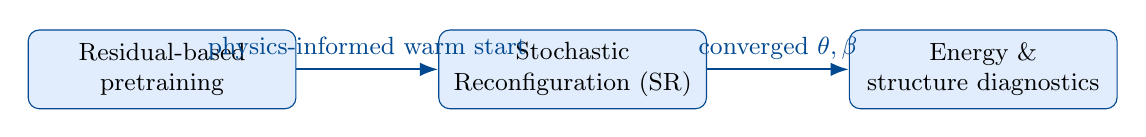
\begin{tikzpicture}[
      box/.style={draw=uioblue,fill=lightblue,rounded corners=4pt,
                  minimum width=3.4cm,minimum height=1.0cm,
                  font=\small,align=center},
      arr/.style={-Latex,thick,uioblue,font=\scriptsize}]
    \node[box] (pre)  {Residual-based\\pretraining};
    \node[box, right=1.8cm of pre] (sr)  {Stochastic\\Reconfiguration (SR)};
    \node[box, right=1.8cm of sr]  (ev)  {Energy \&\\structure diagnostics};
    \draw[arr] (pre) -- (sr)
      node[midway,above]{\small physics-informed warm start};
    \draw[arr] (sr)  -- (ev)
      node[midway,above]{\small converged $\theta,\beta$};
  \end{tikzpicture}
  \end{center}
  \medskip
  \begin{columns}[T]
    \begin{column}{0.48\textwidth}
      \begin{block}{Stage 1 --- Residual pretraining}
        Minimise PINN residual loss enforcing the
        many-body Schr\"odinger equation pointwise at
        collocation points. Provides a
        physically-grounded initialisation.
      \end{block}
    \end{column}
    \begin{column}{0.48\textwidth}
      \begin{block}{Stage 2 --- SR tail}
        Natural gradient on the variational manifold:
        \[
          \delta\theta = -\eta\, S^{-1}\mathbf{g},
          \quad
          S_{ij} = \mathrm{Cov}(O_i,O_j)
        \]
        Quantum geometric tensor as preconditioner.
        Removes residual correlation errors efficiently.
      \end{block}
    \end{column}
  \end{columns}
\end{frame}

% =============================================================================
\section{Results: Ground-State Energies}
% =============================================================================

\begin{frame}{Ground-State Energies: $N=2$ Electrons}
  \begin{columns}[T]
    \begin{column}{0.54\textwidth}
      \begin{block}{$N=2$,\ $\omega\in[0.001,1]$ (Hartree)}
        \small\renewcommand{\arraystretch}{1.25}
        \begin{tabular}{cccr}
          \toprule
          $\omega$ & DMC & PINN+CTNN & \%\,err \\
          \midrule
          $0.01$ & $0.073839(2)$ & $0.0738382(5)$ & $-0.001$ \\
          $0.10$ & $0.44079(1)$  & $0.440796(4)$  & $\phantom{+}0.000$ \\
          $0.50$ & $1.65977(1)$  & $1.65976(1)$   & $-0.001$ \\
          $1.00$ & $3.00000$     & $3.00000(2)$   & $\phantom{+}0.000$ \\
          \bottomrule
        \end{tabular}
      \end{block}
      \medskip
      \begin{itemize}
        \item Both PINN+BF and PINN+CTNN reproduce DMC
              \textbf{at the level of quoted uncertainties}
              across the full confinement range
        \item Confirms the optimisation pipeline
              can find a near-optimal representation
              for the two-electron problem in all regimes
      \end{itemize}
    \end{column}
    \begin{column}{0.43\textwidth}
      \figph{Energy vs.\ $\omega$ for $N=2$\\[4pt]
             PINN+BF and PINN+CTNN\\
             vs.\ DMC reference\\[6pt]
             Log scale on $\omega$-axis\\[4pt]
             Error bars: $1\sigma$ Monte Carlo}
    \end{column}
  \end{columns}
\end{frame}

\begin{frame}{Ground-State Energies: $N=6,12,20$ Electrons}
  \begin{columns}[T]
    \begin{column}{0.58\textwidth}
      \small\renewcommand{\arraystretch}{1.2}
      \begin{tabular}{ccccc}
        \toprule
        $N$ & $\omega$ & DMC & PINN+CTNN & \%\,err \\
        \midrule
        6  & 0.10 & $3.55385(5)$   & $\mathbf{3.55388(5)}$ & $+0.001$ \\
           & 0.50 & $11.78484(6)$  & $\mathbf{11.7847(2)}$ & $\approx0$ \\
           & 1.00 & $20.15932(8)$  & $\mathbf{20.1585(3)}$ & $-0.004$ \\
        \midrule
        12 & 0.10 & $12.26984(8)$  & $\mathbf{12.2718(1)}$ & $\cdots$ \\
           & 0.50 & $39.1596(1)$   & $\mathbf{39.1604(3)}$ & $+0.002$ \\
           & 1.00 & $65.7001(1)$   & $\mathbf{65.69556(5)}$& $-0.007$ \\
        \midrule
        20 & 0.10 & $29.9779(1)$   & $29.9888(2)$          & $+0.036$ \\
           & 0.50 & $93.8752(1)$   & $\mathbf{93.8789(5)}$ & $+0.004$ \\
           & 1.00 & $155.8822(1)$  & $\mathbf{155.8738(7)}$& $-0.002$ \\
        \bottomrule
      \end{tabular}
      \medskip

      \textbf{Bold} = PINN+CTNN lower than PINN+BF
    \end{column}
    \begin{column}{0.38\textwidth}
      \figph{Relative error vs.\ $\omega$\\[4pt]
             $N=6,12,20$\\[4pt]
             PINN+BF (open symbols)\\
             PINN+CTNN (filled symbols)\\[6pt]
             CTNN systematically\\
             closer to DMC for $N\ge6$}
      \medskip
      \small\textcolor{uioblue}{
        Errors $\lesssim 0.04\%$ across\\
        $N=2$--$20$,\ $\omega\in[10^{-3},1]$}
    \end{column}
  \end{columns}
\end{frame}

% =============================================================================
\section{Results: Energy Partitioning and the Wigner Regime}
% =============================================================================

\begin{frame}{Energy Partitioning Diagnostics}
  \[
    E = \vev{T} + \vev{V_\text{int}} + \vev{V_\text{trap}},
    \qquad
    \Gamma(\omega)=\frac{\vev{V_\text{int}}}{\vev{T}},
    \qquad
    \mathcal{C}(\omega)=\frac{2\vev{V_\text{trap}}}{\vev{V_\text{int}}}
  \]
  \begin{columns}[T]
    \begin{column}{0.52\textwidth}
      \small\renewcommand{\arraystretch}{1.25}
      \begin{tabular}{ccccc}
        \toprule
        $N$
          & \multicolumn{2}{c}{$\omega=1$}
          & \multicolumn{2}{c}{$\omega=10^{-3}$} \\
        \cmidrule(lr){2-3}\cmidrule(lr){4-5}
          & $\Gamma$ & $\mathcal{C}$
          & $\Gamma$ & $\mathcal{C}$ \\
        \midrule
        2  & 0.93 & 3.13 & 8.64  & 1.226 \\
        6  & 2.41 & 1.83 & 24.6  & 1.074 \\
        12 & 3.61 & 1.56 & 41.1  & 1.049 \\
        20 & 4.66 & 1.43 & 57.3  & 1.038 \\
        \bottomrule
      \end{tabular}
      \medskip
      \begin{itemize}
        \item $\Gamma\gg1$: interaction-dominated (Wigner)
        \item $\mathcal{C}\to1$: quasi-classical balance;
              $V_\text{int}\approx2V_\text{trap}$
        \item Convergence to $\mathcal{C}=1$ improves with $N$
      \end{itemize}
    \end{column}
    \begin{column}{0.45\textwidth}
      \begin{block}{Physics-based validation}
        Harmonic+Coulomb virial identity:
        \[
          2\vev{T} = 2\vev{V_\text{trap}} - \vev{V_\text{int}}
        \]
        Satisfied to $\lesssim0.4\%$ relative accuracy
        across \emph{all} $(N,\omega)$.\\[4pt]
        Strong internal check where DMC
        benchmarks are unavailable.
      \end{block}
      \medskip
      \small
      RMS radius: $r_\text{rms}=\sqrt{2\vev{V_\text{trap}}/N\omega^2}$\\[4pt]
      At $\omega=10^{-3}$:
      $r_\text{rms}\approx70$, $126$, $171$, $209$\,a.u.\\
      for $N=2,6,12,20$ respectively.\\
      \textcolor{uioblue}{\textbf{Macroscopic Wigner cloud!}}
    \end{column}
  \end{columns}
\end{frame}

\begin{frame}{$\Gamma$ and Cloud Expansion vs.\ Confinement}
  \begin{columns}[T]
    \begin{column}{0.48\textwidth}
      \figph{$\Gamma(\omega)=\vev{V_\text{int}}/\vev{T}$\\
             vs.\ $\omega$ (log--log scale)\\[4pt]
             $N=2,6,12,20$\\[6pt]
             Sharp rise as $\omega\to0$:\\
             crossover to interaction-dominated states\\[4pt]
             e.g.\ $\Gamma: 0.93\to8.64$ for $N=2$}
    \end{column}
    \begin{column}{0.48\textwidth}
      \figph{RMS cloud radius $r_\text{rms}$\\
             vs.\ $\omega$ (log--log scale)\\[4pt]
             $N=2,6,12,20$\\[6pt]
             Rapid expansion as $\omega\to0$:\\
             interaction-driven swelling\\
             into the Wigner regime}
    \end{column}
  \end{columns}
\end{frame}

% =============================================================================
\section{Results: Wigner Molecule Formation}
% =============================================================================

\begin{frame}{One-Body Densities: Visual Crossover}
  \begin{columns}[T]
    \begin{column}{0.48\textwidth}
      \begin{center}\textbf{Strong confinement ($\omega=1$)}\end{center}
      \figph{$\rho_1(\mathbf{r})$ for $N=2,6,12,20$\\at $\omega=1.0$\\[6pt]
             Compact, isotropic density.\\
             Increasing $N$ fills the trap.\\
             No ring structure.}
    \end{column}
    \begin{column}{0.48\textwidth}
      \begin{center}\textbf{Weak confinement ($\omega=0.001$)}\end{center}
      \figph{$\rho_1(\mathbf{r})$ for $N=2,6,12,20$\\at $\omega=0.001$\\[6pt]
             Broad density with\\pronounced radial rings.\\
             Strong Coulomb localisation.}
    \end{column}
  \end{columns}
\end{frame}

\begin{frame}{Shell Topology: Discrete Wigner Patterns}
  \begin{columns}[T]
    \begin{column}{0.52\textwidth}
      \begin{block}{Label-invariant shell occupancies}
        \small\renewcommand{\arraystretch}{1.25}
        \begin{tabular}{cccc}
          \toprule
          $N$ & $\omega=10^{-3}$ & $\omega=10^{-2}$ & $\omega=1$ \\
          \midrule
          2  & (2)              & (2)              & (2)    \\
          6  & (1,5)            & (1,5)            & (6)    \\
          12 & \textbf{(3,9)}   & (1,11)           & (1,11) \\
          20 & \textbf{(1,7,12)}& (1,19)           & (1,19) \\
          \bottomrule
        \end{tabular}
      \end{block}
      \medskip
      \begin{itemize}
        \item At $\omega=10^{-3}$: classical finite-$N$ Wigner patterns
        \item \textbf{Sharp topology collapse} at $\omega=10^{-2}$
              for $N=12$ and $N=20$:
              $(3,9)\to(1,11)$ and $(1,7,12)\to(1,19)$
        \item $N=6$: two-ring structure persists to $\omega\le0.1$
      \end{itemize}
    \end{column}
    \begin{column}{0.44\textwidth}
      \figph{Schematic of shell patterns:\\[4pt]
             $(2)$ --- $N=2$\\
             $(1,5)$ --- $N=6$\\
             $(3,9)$ --- $N=12$\\
             $(1,7,12)$ --- $N=20$\\[6pt]
             at $\omega=10^{-3}$\\[4pt]
             Finite-$N$ Wigner molecules}
    \end{column}
  \end{columns}
\end{frame}

\begin{frame}{Shell Radii, Separation Gaps, and Angular Order}
  \begin{columns}[T]
    \begin{column}{0.50\textwidth}
      \begin{block}{Shell radii and inter-shell gaps (a.u.)}
        \small\renewcommand{\arraystretch}{1.2}
        \begin{tabular}{cccccc}
          \toprule
          $N$ & $\omega$ & occ. & $r_0$ & $r_1$ & gap$_{01}$ \\
          \midrule
          6  & $10^{-3}$ & (1,5)  & 35.6 & 135.7 & 100.1 \\
             & $10^{-2}$ & (1,5)  & 13.3 & 29.6  & 16.3  \\
             & $1$       & (6)    & 1.50 & ---   & ---   \\
          \midrule
          12 & $10^{-3}$ & (3,9)  & 77.1 & 189.4 & 112.3 \\
             & $10^{-2}$ & (1,11) & 10.3 & 37.7  & 27.3  \\
             & $1$       & (1,11) & 0.55 & 2.00  & 1.46  \\
          \midrule
          20 & $10^{-3}$ & (1,7,12)&38.0 & 132.0 & 94.0  \\
             & $1$       & (1,19) & 0.55 & 2.32  & 1.76  \\
          \bottomrule
        \end{tabular}
      \end{block}
      \small Gap collapse mirrors topology transition
    \end{column}
    \begin{column}{0.46\textwidth}
      \begin{block}{Rotation-registered angular order}
        \[
          \Phi_{s,\text{reg}}
          = \Bigl\langle
            \Bigl|\tfrac{1}{n_s}
            \textstyle\sum_{j\in s}
            e^{i n_s\theta^{\text{reg}}_j}\Bigr|
            \Bigr\rangle_t
        \]
        \small
        \textbf{Internal} (registered) vs.\ lab-frame order:\\[2pt]
        \begin{tabular}{ccccc}
          \toprule
          $N$ & $\omega$ & occ. & $\tilde C_\text{gl}$ & $C_\text{gl}$ \\
          \midrule
          12 & $10^{-3}$ & (3,9)    & \textbf{1.068} & 0.021 \\
          12 & $10^{-2}$ & (1,11)   & 0.276 & 0.005 \\
          20 & $10^{-3}$ & (1,7,12) & \textbf{0.791} & 0.056 \\
          20 & $10^{-2}$ & (1,19)   & 0.203 & 0.000 \\
          \bottomrule
        \end{tabular}
      \end{block}
      \small $C_\text{gl}\ll\tilde C_\text{gl}$: global rotation,
      not absence of internal order
    \end{column}
  \end{columns}
\end{frame}

\begin{frame}{Lindemann Disorder and Mode-Alignment Diagnostic}
  \begin{columns}[T]
    \begin{column}{0.50\textwidth}
      \begin{block}{Lindemann disorder $L_{s,\text{reg}}$}
        \small Relative positional fluctuations per shell.
        Larger $=$ more disordered.
        \smallskip
        \renewcommand{\arraystretch}{1.1}
        \begin{tabular}{ccccc}
          \toprule
          $N$ & $\omega$ & occ. & $L_\text{in}$ & $L_\text{out}$ \\
          \midrule
          12 & $10^{-3}$ & (3,9)    & 0.274 & 0.255 \\
          12 & $10^{-2}$ & (1,11)   & ---   & 0.450 \\
          12 & $1$       & (1,11)   & ---   & 0.618 \\
          20 & $10^{-3}$ & (1,7,12) & 0.351 & 0.270 \\
          20 & $1$       & (1,19)   & ---   & 0.692 \\
          \bottomrule
        \end{tabular}
        \smallskip

        \small Stiff rings at $\omega=10^{-3}$;
        progressive melting as $\omega\uparrow$
      \end{block}
    \end{column}
    \begin{column}{0.47\textwidth}
      \begin{block}{Mode-alignment diagnostic}
        \small Compare empirical covariance $C$ to Hessian $H$
        of classical equilibrium (trap + Coulomb):
        \begin{itemize}\small
          \item $\|[C,H]\|$ smallest at $\omega=10^{-3}$
          \item Variance concentrated in soft-mode subspace
          \item Fluctuations are ``molecule-like'', not fluid-like
        \end{itemize}
      \end{block}
      \vspace{6pt}
      \figph[0.97\linewidth]{Commutator norm $\|[C,H]\|$\\and soft-mode\\overlap weight vs.\ $\omega$\\[4pt]
             $N=6,12,20$}
    \end{column}
  \end{columns}
\end{frame}

\begin{frame}{Pair-Statistics Validation: Angular Order Beyond Shelling}
  \begin{columns}[T]
    \begin{column}{0.54\textwidth}
      \textbf{Question:} is the observed structure genuinely polygonal,
      or merely a radial-shelling artefact?
      \medskip
      \begin{block}{Two generative models (same shell radii)}
        \begin{enumerate}\small
          \item \textbf{Polygon model}: regular $n_s$-gons per shell,
                optimally phase-aligned
          \item \textbf{Uniform-angle model}: same radii,
                no angular order
        \end{enumerate}
        Compare cosine similarity of each model to the
        empirical pair-distance histogram.
      \end{block}
      \medskip
      \[
        \Delta\cos = \cos_\text{poly} - \cos_\text{uni}
      \]
      \begin{itemize}\small
        \item $\Delta\cos > 0$ isolates \emph{genuine angular correlations}
        \item Largest gain at \emph{weakest} confinement
        \item Decreases monotonically with $\omega$
        \item Confirms the Wigner-molecule interpretation
      \end{itemize}
    \end{column}
    \begin{column}{0.42\textwidth}
      \figph{$\Delta\cos$ vs.\ $\omega$\\[4pt]
             $N=6,\,12,\,20$\\[6pt]
             Polygon model gain\\
             over uniform-angle\\
             baseline}
    \end{column}
  \end{columns}
\end{frame}

% =============================================================================
\section{Summary and Outlook}
% =============================================================================

\begin{frame}{Summary: Seven Diagnostics, One Consistent Picture}
  \begin{block}{Multi-diagnostic Wigner crossover as $\omega\to0$}
    \footnotesize\renewcommand{\arraystretch}{1.1}
    \begin{tabular}{ll}
      \toprule
      \textbf{Diagnostic} & \textbf{Key finding} \\
      \midrule
      Ground-state energies & $\lesssim0.04\%$ vs.\ DMC,
                              $N=2$--$20$,\ $\omega\in[10^{-3},1]$ \\
      Energy partitioning   & $\Gamma\gg1$, $\mathcal{C}\to1$; virial identity satisfied \\
      One-body densities    & Compact at $\omega=1$; ring formation at $\omega=10^{-3}$ \\
      Shell topology        & Discrete Wigner patterns; sharp collapse at $\omega=10^{-2}$ \\
      Shell radii and gaps  & Macroscopic ($\sim10^2$ a.u.) in Wigner regime \\
      Angular order         & Strong polygon-like \emph{internal} order; global rotation present \\
      Lindemann / modes     & Stiff rings; fluctuations align with classical soft modes \\
      Pair statistics       & Polygon model $>$ uniform-angle; gain largest at small $\omega$ \\
      \bottomrule
    \end{tabular}
  \end{block}
  \smallskip
  \begin{columns}[T]
    \begin{column}{0.48\textwidth}
      \begin{exampleblock}{CTNN vs.\ BF backflow}
        \small CTNN consistently achieves lower energies for $N\ge6$.
        Richer node/edge feature representation captures
        nodal geometry more accurately at scale.
      \end{exampleblock}
    \end{column}
    \begin{column}{0.48\textwidth}
      \begin{exampleblock}{Method validation}
        \small Virial identity + energy closure provide
        \emph{physics-based} checks for all $(N,\omega)$,
        including regimes without DMC benchmarks.
      \end{exampleblock}
    \end{column}
  \end{columns}
\end{frame}

\begin{frame}{Conclusions}
  \begin{itemize}
    \setlength\itemsep{8pt}
    \item Physics-informed neural networks provide a \textbf{continuous-space,
          basis-free framework} for quantum dot many-body physics ---
          no basis truncation, natural fit for arbitrary geometries
    \item The \textbf{Slater--Jastrow--neural correlator} ansatz (PINN+CTNN)
          achieves $\lesssim0.04\%$ error relative to DMC
          across $N=2$--$20$,\ $\omega\in[10^{-3},1]$
    \item \textbf{Residual pretraining + SR} is an effective two-stage pipeline
          combining PINN physical initialisation with variational convergence
    \item A \textbf{seven-diagnostic structural analysis} gives a consistent,
          quantitative picture of the Wigner molecule crossover
    \item \textbf{CTNN backflow outperforms BF} for $N\ge6$:
          richer nodal geometry representations matter at scale
    \item Internal virial and energy-closure checks validate
          results in regimes where external benchmarks are unavailable
  \end{itemize}
\end{frame}

\begin{frame}{Outlook}
  \begin{columns}[T]
    \begin{column}{0.54\textwidth}
      \textbf{Near-term physics goals:}
      \begin{itemize}
        \item Excited states and optical response spectra
        \item Real-time dynamics: quench protocols, Kondo physics
        \item Anisotropic and multi-dot (double-dot) geometries
        \item Scale CTNN towards $N\sim50$--$100$
      \end{itemize}
      \medskip
      \textbf{Methodological directions:}
      \begin{itemize}
        \item Adaptive collocation and importance sampling
        \item Equivariant architectures beyond permutation symmetry
        \item Hybrid PINN--VMC strategies
        \item Integration with quantum simulation platforms
      \end{itemize}
    \end{column}
    \begin{column}{0.42\textwidth}
      \figph{Roadmap diagram:\\[4pt]
             PINN framework\\
             $\downarrow$\\
             Excited states\\
             $\downarrow$\\
             Real-time dynamics\\
             $\downarrow$\\
             Larger $N$, device design\\
             $\downarrow$\\
             Quantum hardware integration}
    \end{column}
  \end{columns}
\end{frame}

\begin{frame}[plain]
  \begin{tikzpicture}[remember picture, overlay]
    \fill[uioblue] (current page.north west) rectangle (current page.south east);
    \node[white, font=\LARGE\bfseries] at (current page.center)
      {Thank you --- questions welcome};
    \node[white, font=\large, below=1.4cm of current page.center]
      {\texttt{morten.hjorth-jensen@fys.uio.no}};
    \node[white, font=\normalsize, below=2.2cm of current page.center]
      {Department of Physics \& CCSE, University of Oslo};
  \end{tikzpicture}
\end{frame}

\end{document}
